\section{Introduction}
\label{sec:intro}

%\KZ{Our premise: Review sentences tend to be short and informative. It is our belief
%that every sentence in a review should provide some useful info.}

Abstractive opinion summarization is the process of 
producing a summary for a set of 
subjective user reviews about an entity, which can be 
a place, a product, a service or a movie. 
Such a set of reviews is called a {\em multi-review} in this paper. 
Deep learning (DL) techniques have made great successes 
in opinion summarization
~\cite{NallapatiZSGX16,SeeLM17,LiuLZ18,CelikyilmazBHC18,BART20,liu2021keyword,multisumSIG21}, 
which require training on a large number of document-summary pairs.
Unfortunately, opinion summarization tasks
generally lack the training pairs with multi-review as input and reference summary as output,
as it is difficult and costly for annotators to write summaries for 
multi-reviews on a large scale.

In view of the above challenge, some approaches~\cite{MeanSum19,Copycat20,tree21}
adopt unsupervised learning, e.g., by using the auto-encoders.
They reconstruct individual reviews by encoding themselves
at training time, 
which may prevent them from effectively generating summary by encoding multi-review at test time.
Because the multi-review, including much redundant information, is actually the noisy version of summary.
Other more popular approaches~\cite{Denoise20,Fewshot20,Plansum20,transsum21} 
focus on creating synthetic (multi-review, summary) pairs for training.
They typically sample one or more reviews from all reviews 
about an entity
as the ``pseudo'' summary, that is, the output of the synthetic training pair.
These approaches differ from each other by how the input is created.
Existing approaches use either {\em textual} or  {\em structured} information (see \tabref{tab:previous_data})
to create the input.

\begin{table}[th]
	\centering
	\small
		\begin{tabular}{|m{7.8cm}<{\centering}|}
			\hline 
			\rule{0pt}{10pt} \bf Synthetic Output (a sampled review)\\
			\hline
			\makecell[l]{very \textbf{disappointed} in \textbf{food} and \textbf{service} . the \textbf{beef} was \textbf{burned} . \\ 
				\textit{the \textbf{staff} \textbf{dismissed} my comments . }} 
					\vspace{0.2em}\\
			\hline
			\end{tabular}
			\begin{tabular}{|p{1.4cm}|m{0.3cm}<{\centering}|p{5.4cm}|}
			\hline
			\multicolumn{3}{|c|}{\rule{0pt}{10pt} \bf Synthetic Input (to be summarized)}  \\	
			\hline
			\multicolumn{3}{|l|}{\bf Textual} \\
			\hline
			\multirow{3}{0.1cm}{\em Random\cite{Fewshot20}} & $R_1$ & very average spanish \textbf{food} .
			\\
			%\cline{2-3}
			& $R_2$ &definitely not a peruvian restaurant
			.
			\\
			%\cline{2-3}
			& $R_3$ &love this place! location is great
			.
			\\ 
			\hline
			\multirow{3}{0.1cm}{\em Similarity~\cite{Plansum20}} & $R_1$ & bad \textbf{food} and \textbf{service} . \textbf{disappointed} \\
			%\cline{2-3}
			& $R_2$& the \textbf{food} and \textbf{service} was not good . very \textbf{bad experience} .
			\\
			%\cline{2-3}
			& $R_3$ &awful \textbf{food} and \textbf{service} . the \textbf{staff} was unfriendly .
			\\
			\hline
			\multicolumn{3}{|l|}{\bf Structured} \\
			\hline
			OpiDig~\cite{OpiDig20}& $OA$ & \textbf{disappointed}, \textbf{food; disappointed}, \textbf{service; burned}, \textbf{beef}
			\\
			\hline
		\end{tabular}
	\caption{Synthetic training pairs (Input, Output) constructed by different methods with 
different input but the same output. 
		Matched words in both the input and the output are bolded.
		$R$ denotes a textual input review. 
		$OA$ denotes explicit opinion-aspect pairs extracted from output.
		The italicized sentence doesn't contain explicit OAs, 
		which is called ``implicit sentence'' (IS).
		``;'' delimits OAs.
	}\label{tab:previous_data}  
\end{table}

%\begin{figure}[th]
%	\centering
%	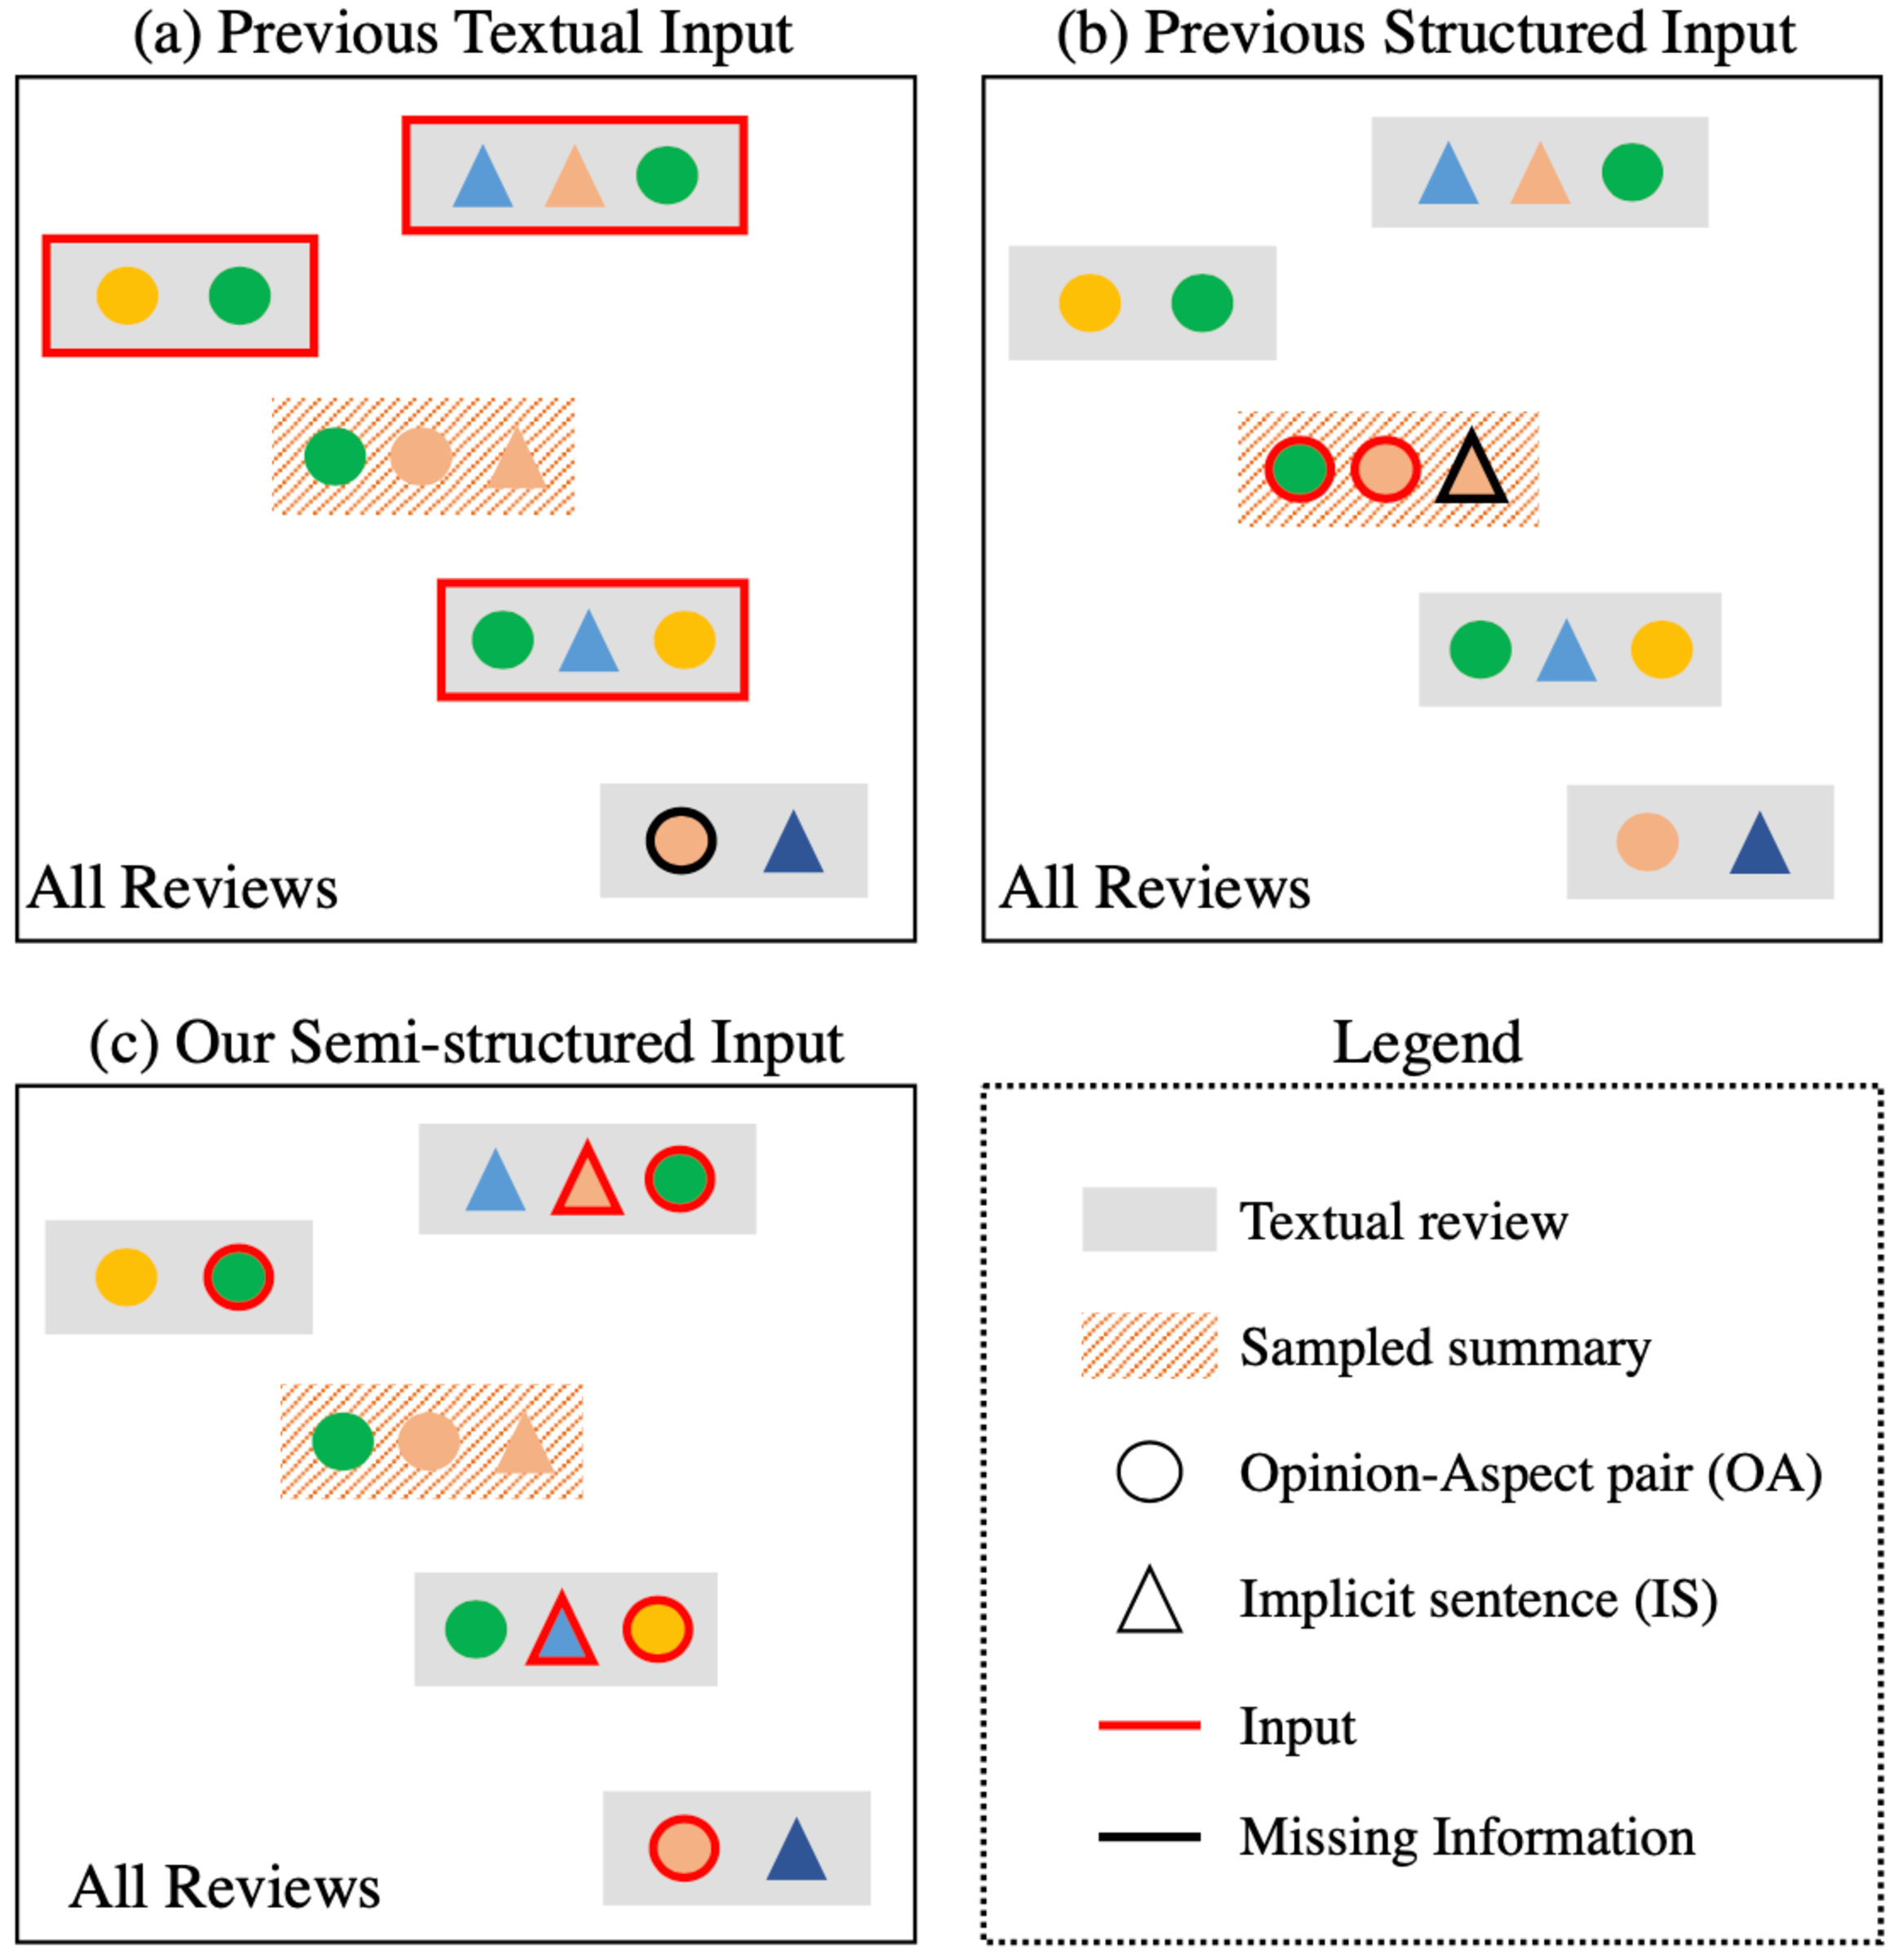
\includegraphics[width=0.85\linewidth]{./brief.pdf}
%	\caption{Different synthetic inputs of the same summary.
%	}
%	\label{fig:brief}
%\end{figure}
\cut{%%%%%%
\begin{table}[th]
	\centering
	\small
    \subtable[Output (sampled summary) with its OAs and ISs]{
	\begin{tabular}{|m{0.3cm}<{\centering}|p{7.1cm}|}
		\hline 
		%\rule{0pt}{10pt}
		\multicolumn{2}{|c|}{\rule{0pt}{10pt} \bf Output} \\
		\hline
		S & \makecell[l]{very \textbf{disappointed} in \textbf{food} and \textbf{service} . the \textbf{beef} was \\ \textbf{burned} . 
				\underline{the \textbf{staff} \textbf{dismissed} my comments .} } 
		\vspace{0.2em}\\
		\hline
		OA & \textbf{disappointed}, \textbf{food; disappointed}, \textbf{service; burned}, \textbf{beef} \\
		\hline
		IS   & the \textbf{staff} \textbf{dismissed} my comments . \\
		\hline
	\end{tabular}
}
\qquad
\subtable[Synthetic input based on summary in (a)]{
	\begin{tabular}{|m{0.9cm}|m{0.3cm}<{\centering}|m{5.8cm}|}
		\hline
		\multicolumn{3}{|c|}{\rule{0pt}{10pt} \bf Input}  \\	
		\hline
		\multicolumn{3}{|l|}{\bf Textual} \\
		\hline
		\multirow{3}{0.1cm}{FewSum} & $R_1$ & very average spanish \textbf{food} .
		\\
		\cline{2-3}
		& $R_2$ &definitely not a peruvian restaurant
		.
		\\
		\cline{2-3}
		& $R_3$ &love this place! location is great
		.
		\\
		\hline
		\multirow{3}{0.1cm}{Denoise} & $R_1$ & very uncomfortable in \textbf{food} and \textbf{staff} . the \textbf{ food} was bad . the \textbf{staff} ignored me .
		\\
		\cline{2-3}
		& $R_2$ & bad \textbf{food} . the \textbf{staff} ignored me . very uncomfortable in restaurant .\\
		\cline{2-3}
		& $R_3$ &I was \textbf{disappointed} with the restaurant. the \textbf{food} was not bad . but the \textbf{staff} was unfriendly .
		\\
		\hline
		\multirow{3}{0.1cm}{PlanSum} & $R_1$ & bad \textbf{food} and \textbf{service} . \textbf{disappointed} \\
		\cline{2-3}
		& $R_2$& the \textbf{food} and \textbf{service} was not good . very \textbf{bad experience} .
		\\
		\cline{2-3}
		& $R_3$ &awful \textbf{food} and \textbf{service} . the \textbf{staff} was unfriendly .
		\\
		\hline
		\multicolumn{3}{|l|}{\bf Structured} \\
		\hline
		OpiDig & OA & \textbf{disappointed}, \textbf{food; disappointed}, \textbf{service; burned}, \textbf{beef}
		\\
		\hline
		\multicolumn{3}{|l|}{\bf Semi-structured} \\
		\hline
		\multirow{2}{0.1cm}{Ours} & OA &not good, \textbf{food;} great, location\textbf{;} bad, \textbf{food; disappointed}, \textbf{service;} not fresh, \textbf{beef;} unfriendly, \textbf{staff;} awful, \textbf{service}\\
		\cline{2-3}
		& IS &not recommended\textbf{;} my questions were \textbf{dismissed} .\textbf{;} the \textbf{staff} ignored our \textbf{comments} .\\
		\hline
	\end{tabular}
}
	\caption{The synthetic training pairs (Input, Output) constructed by different methods with the same summary as output. 
		Bolded words in the input and output are matched.
	   $S$ is the output summary. 
	   $R$ denotes a textual input review. 
		The underlined sentences don't contain explicit opinion-aspect pairs (OA), 
		which are called ``implicit sentences'' (IS).  
		%$R$ is textual review, OA is opinion-aspect pair and IS is implicit sentence. 
		``;'' delimits OAs and ISs in our method.
		}\label{tab:previous_data}  
\end{table}
}%%%%%%

The {\em textual} input is usually a set of reviews sampled 
from all reviews in the corpus. 
The most straight-forward method is {\em leave-one-out}~\cite{Copycat20}, 
which samples one review as the summary and takes the rest as the input. 
TranSum~\cite{transsum21} improves {\em leave-one-out} by weighting 
each input review using its similarity to the summary.
However, these methods result in very long textual input, not only costing more memory to process but also introducing noises 
because the inputs of different summaries of the same entity are almost identical except for one review.
An alternative to {\em leave-one-out} is to sample (or synthesize) several 
original reviews from all reviews, 
either randomly 
~\cite{Fewshot20}, or by the similarity between the input text and the summary 
~\cite{Denoise20,Plansum20}.
Their downsides are: i) the content of summary and its input may be completely unrelated, 
like the input of {\em Random} row in \tabref{tab:previous_data}; 
ii) certain important information in the summary can be missing from the input: ``beef'' in the summary 
does not appear in the input of {\em Similarity} row in \tabref{tab:previous_data}.
This is because some information in the summary is not so popular in all reviews or
not the most important in one review,
causing the reviews containing such information to be not sampled.
%to be neglected by the sampling process.


Previous works have acknowledged that when summarizing opinion reviews, the most critical information
to be considered are aspects of the product or service that appear in the reviews,
and opinions about these aspects~\cite{AngelidisL18,MukherjeePVGBG20}.
Hence it is natural to consider extracting the {\em structured} information, 
that is, opinion-aspect pairs (OAs) such as (burned, beef) and (disappointed, service),
from the reviews first, and then doing summarization.
OpiDig~\cite{OpiDig20} is a self-supervised seq2seq model, which uses a review as output 
while extracting OAs from this review as input.
At inference time, OpiDig clusters the OAs 
of multi-reviews and selects those pairs in the center as input to 
generate a summary. 
However, even with the state-of-the-art OA extraction algorithm,%~\cite{MiaoLWT20}, 
it is not easy to extract OAs from some sentences, such as the italicized sentence 
about ``staff'' in \tabref{tab:previous_data}. 
We call these sentences ``implicit sentences'' (ISs).
As \tabref{tab:previous_data} shows, OpiDig cannot learn to produce the implicit sentence in the output 
by only taking OAs as the input.


In this paper, we propose to use semi-structured data, 
instead of only textual or structured reviews as the input of our synthetic training data. 
Most reviews in the opinion summarization are mainly explicit opinions supplemented by some detailed description.
For a review, its OAs express the opinion explicitly
and ISs express the opinion implicitly through the description of specific information.
As reviews tend to be short and informative,
we believe that every sentence in them provides some useful information and should not be neglected.
To this end, our semi-structured input is a combination of OAs and ISs, as shown in \tabref{tab:ours_data}.

\begin{table}[th]
	\centering
	\small
		\begin{tabular}{|p{0.4cm}<{\centering}p{7.2cm}|}
			\hline 
			%\rule{0pt}{10pt}
			\multicolumn{2}{|c|}{\rule{0pt}{10pt} \bf Output (Sampled summary)} \\
			\hline
		    \multicolumn{2}{|c|}{\makecell[l]{very \textbf{disappointed} in \textbf{food} and \textbf{service} . the \textbf{beef} was  \textbf{burned} . \\
		    		the \textbf{staff} \textbf{dismissed} my comments . } } \\
			\hline
			\hline
			\multicolumn{2}{|c|}{\rule{0pt}{10pt} \bf Semi-structured Output} \\
			\hline
			$OA$ & \textbf{disappointed}, \textbf{food; disappointed}, \textbf{service; burned}, \textbf{beef} \\
			%\hline
			$IS$   & the \textbf{staff} \textbf{dismissed} my comments . \\
			\hline
		%\end{tabular}	
		%\begin{tabular}{|m{0.4cm}<{\centering}|m{7.2cm}|}
			\hline
			\multicolumn{2}{|c|}{\rule{0pt}{10pt} \bf Semi-structured Input}  \\	
			\hline
			$OA$ &not good, \textbf{food;} great, location\textbf{;} bad, \textbf{food; disappointed}, \textbf{service;} not fresh, \textbf{beef;} unfriendly, \textbf{staff;} awful, \textbf{service}\\
			%\hline
			$IS$ &not recommended .\textbf{;} my questions were \textbf{dismissed} .\textbf{;} the \textbf{staff} ignored our \textbf{comments} .\\
			\hline
		\end{tabular}
	\caption{Synthetic training pair constructed by our approach. In this paper, we take (semi-structured input, output) as training pair. 
		``;'' delimits OAs and ISs.
	}\label{tab:ours_data}  
\end{table}

We create a synthetic training dataset by 
first sampling a textual review as a pseudo summary (output).
Since in the real-world scenario,
any input multi-review may contain redundancies and contradictions that should not
be summarized, we introduce noises into the input by sampling OAs and ISs from all reviews about an entity 
except for the one chosen as the output summary.
As shown in \tabref{tab:ours_data}, 
semi-structured input is the noisy version of the semi-structured output, which can cover the information in output.
Compared with taking multiple textual 
reviews or OAs extracted from a single review as input,
our noisy OAs and ISs %selected from all reviews 
make the synthetic pair more realistic
and help the model learn to identify important aspects and opinions from redundant information.

In order to capture explicit opinions (opinion-aspect pairs) 
and implicit opinions (implicit sentences) at the same time,
we propose an aspect-guided model with an OA encoder and
an IS encoder. 
We first pretrain a single encoder model variation by taking only noisy OAs as input, 
which learns to select important OAs and make sentences through the selected OAs. 
Then, we initialize the aspect-guided model with the pretrained OA encoder and 
then train its dual encoder by taking both OAs and ISs as input.
In this way, our model not only allows the information of OA and IS to complement each other but also pays more attention to explicit opinions that are more important in opinion summarization,
leading to reduce information missing from generated summaries.

In summary, our contributions are as follows:
\begin{enumerate}
\item We convert textual or structured input in previous synthetic datasets to semi-structured input by extracting OAs and ISs from previous input and discover that semi-structured input is more effective in capturing opinions.
(\figref{fig:abl_data})

\item 
We propose a new data creation method to construct semi-structured synthetic training pair by first sampling a review as summary and then sampling noisy OAs and ISs from other reviews as input according to the summary.
We also design an aspect-guided model for semi-structured data to generate high-quality summaries.
(\secref{sec:approach})

\item 
Compared with previous opinion summarization systems, 
the proposed model trained on our synthetic dataset substantially outperforms the 
state-of-the-art methods on the Yelp, Amazon and RottenTomatos datasets. (\tabref{tab:all})
\end{enumerate}
